
\subsection{引子}

\begin{NOTE}{BZOJ - 2286 消耗战}{}

\end{NOTE}


\vskip 0.2 in
\texttt{
### Description\\\\在一场战争中,战场由 $n$ 个岛屿和 $n-1$ 个桥梁组成,保证每两个岛屿间有且仅有一条路径可达。现在,我军已经侦查到敌军的总部在编号为 $1$ 的岛屿,而且他们已经没有足够多的能源维系战斗,我军胜利在望。已知在其他 $k$ 个岛屿上有丰富能源,为了防止敌军获取能源,我军的任务是炸毁一些桥梁,使得敌军不能到达任何能源丰富的岛屿。由于不同桥梁的材质和结构不同,所以炸毁不同的桥梁有不同的代价,我军希望在满足目标的同时使得总代价最小。\\\\侦查部门还发现,敌军有一台神秘机器。即使我军切断所有能源之后,他们也可以用那台机器。机器产生的效果不仅仅会修复所有我军炸毁的桥梁,而且会重新随机资源分布(但可以保证的是,资源不会分布到 $1$ 号岛屿上)。不过侦查部门还发现了这台机器只能够使用 $m$ 次,所以我们只需要把每次任务完成即可。\\\\### Input\\\\第一行一个整数 $n$,代表岛屿数量。\\\\接下来 n-1 行,每行三个整数 $u,v,w$,代表 $u$ 号岛屿和 $v$ 号岛屿由一条代价为 $c$ 的桥梁直接相连,保证 $1\le u,v\le n$ 且 $1\le c\le 10^5$。\\\\第 $n+1$ 行,一个整数 $m$,代表敌方机器能使用的次数。\\\\接下来 $m$ 行,每行一个整数 $k_i$,代表第 $i$ 次后,有 $k_i$ 个岛屿资源丰富,接下来 $k$ 个整数 $h_1,h_2,\cdots ,h_k$,表示资源丰富岛屿的编号。\\\\### Output\\\\输出有 $m$ 行,分别代表每次任务的最小代价。\\\\### Sample Input\\\\```text\\10\\1 5 13\\1 9 6\\2 1 19\\2 4 8\\2 3 91\\5 6 8\\7 5 4\\7 8 31\\10 7 9\\3\\2 10 6\\4 5 7 8 3\\3 9 4 6\\```\\\\### Sample Output\\\\```text\\12\\32\\22\\```\\\\### HINT\\\\对于 $100\%$ 的数据,$2\le n\le 2.5\times 10^5,m\ge 1,\sum k_i\le 5\times 10^5,1\le k_i\le n-1$。\\\\### Source\\\\[Stage2 day2](http://www.lydsy.com/JudgeOnline/problemset.php?search=Stage2%20day2)}
\vskip 0.2 in

\subsection{虚树 Virtual Tree}

对于上面那题,我们不难发现——如果树的点数很少,那么我们可以直接跑 DP。

首先我们称某次询问中被选中的点为——\textbf{「关键点」}。

设 $Dp[i]$ 表示——使 $i$ 不与其子树中任意一个关键点联通的\textbf{最小代价}。

设 $w[a,b]$ 表示 $a$ 与 $b$ 之间的边的权值。

则:

\begin{itemize}
\item 若 $son[i]$ 不是关键点:$Dp[i]=Dp[i] + \min \{Dp[son[i]],w[i,son[i]]\}$;
\item 若 $son[i]$ 是关键点:$Dp[i]=Dp[i] + w[i,son[i]]$。
\end{itemize}

很好,这样我们得到了一份 $O(n\times q)$ 的代码。

听起来很有意思。

我们不难发现——其实很多点是没有用的。

比如下图:

\begin{figure}[h]
\centering
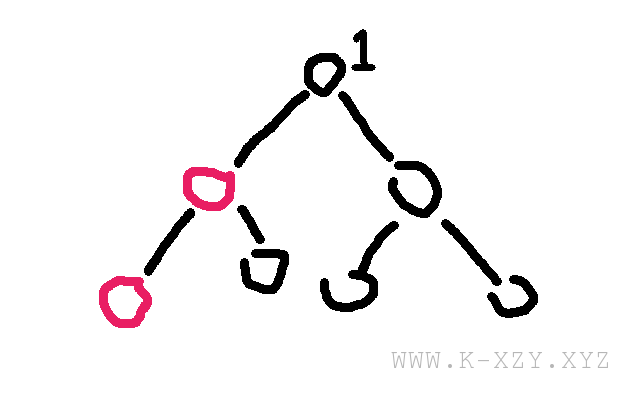
\includegraphics[width=0.5\textwidth]{images/vtree1.png} 
\caption{vtree1}
\end{figure}

图中只有两个红色的点是\textbf{关键点},而别的黑色的点全都是「非关键点」。一号节点(敌人所在之处)是树顶的那个标了 $1$ 的节点。

对于这题来说,我们只需要保证红色的点无法到达 $1$ 号节点就行了。

通过肉眼观察可以得出结论——$1$ 号节点的右子树(虽然实际上可能有多个子树,但这里只有两个子树,所以暂时这么称呼了)一个红色节点都木有,\textbf{所以没必要去 DP 它},不是吗?

观察题目给出的条件,红色点(关键点)的总数是与 $n$ 同阶的,也就是说实际上一次询问中红色的点对于整棵树来说是很稀疏的,所以如果我们能让复杂度由红色点的总数来决定就好了。

因此我们需要\textbf{浓缩信息,把一整颗大树浓缩成一颗小树}。

由此我们引出了\textbf{「虚树」}这个概念。

我们先直观地来看看虚树的样子。

下图中,左边为原树,右边为生成的新的虚树。

\begin{figure}[h]
\centering
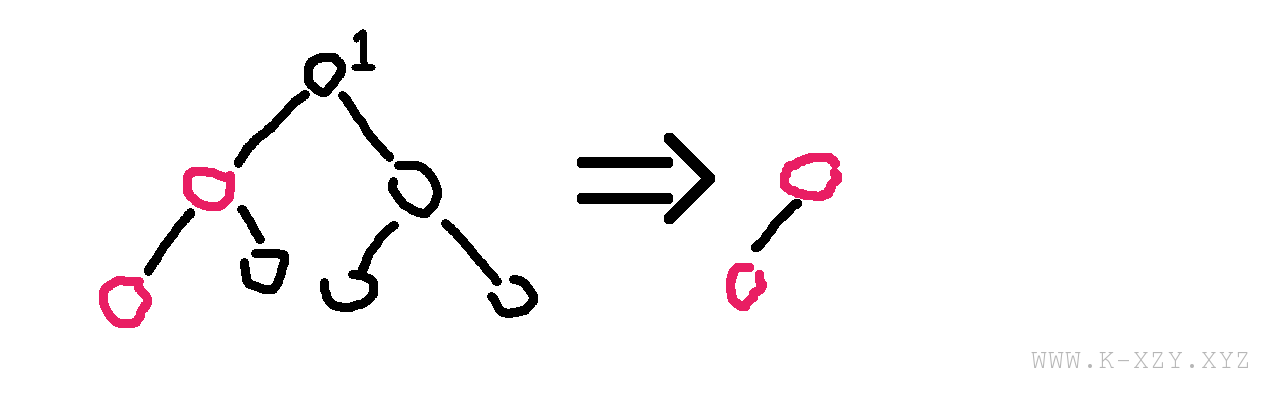
\includegraphics[width=0.5\textwidth]{images/vtree2.png} 
\caption{vtree2}
\end{figure}

\begin{figure}[h]
\centering
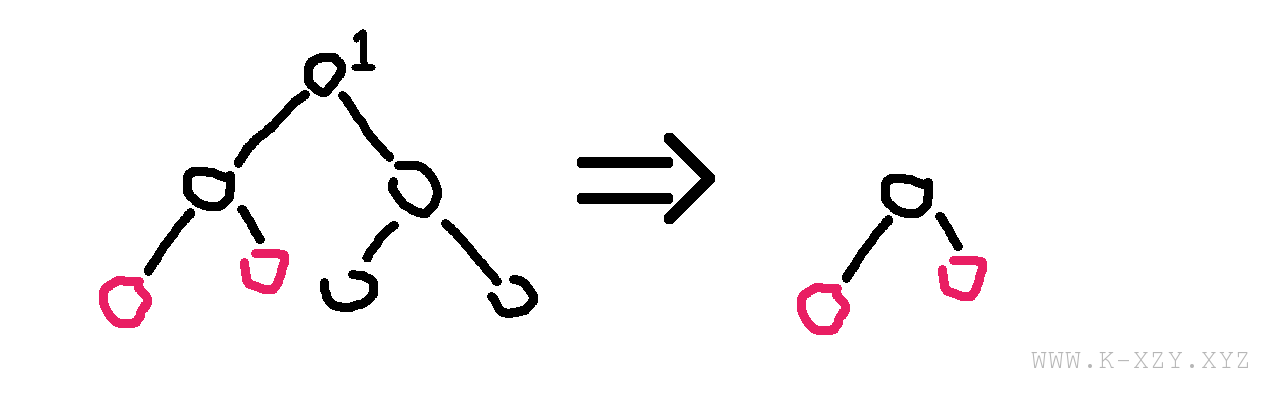
\includegraphics[width=0.5\textwidth]{images/vtree3.png} 
\caption{vtree3}
\end{figure}

\begin{figure}[h]
\centering
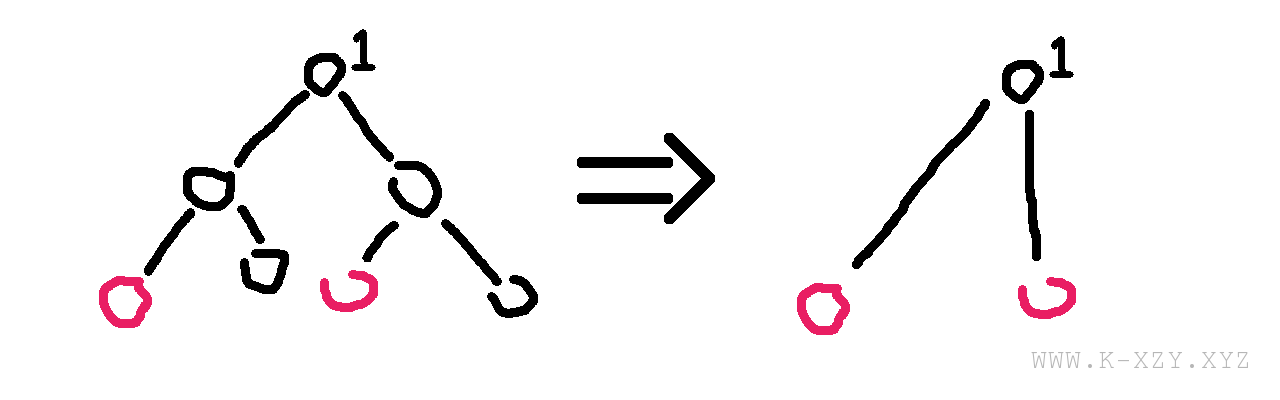
\includegraphics[width=0.5\textwidth]{images/vtree4.png} 
\caption{vtree4}
\end{figure}

\begin{figure}[h]
\centering
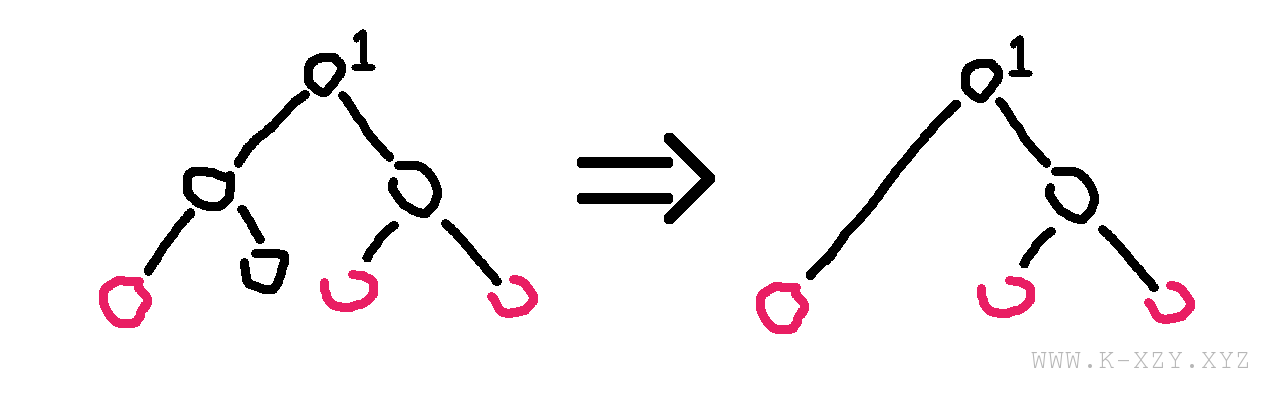
\includegraphics[width=0.5\textwidth]{images/vtree5.png} 
\caption{vtree5}
\end{figure}

看明白了吗?

因为任意两个关键点的 LCA 也是需要保存重要信息的,所以我们需要保存它们的 LCA,也就是虚树中不一定只有关键点。

不难发现虚树中祖先 -> 后代的关系并不会改变。(就是不会出现原本 $a$ 是 $b$ 的祖先结果后面 $a$ 变成 $b$ 的后代了之类的鬼事)

但我们不可能 $O(k^2)$ 暴力枚举 LCA,所以我们不难想到——首先将关键点按 DFS 序排序,然后排完序以后相邻的两个关键点(相邻指的是在排序后的序列中下表差值的绝对值等于 1)求一下 LCA,并把它加入虚树。

因为可能多个节点的 LCA 可能是同一个,所以我们不能多次将它加入虚树。

非常直观的一个方法是:

\begin{itemize}
\item 将关键点按 DFS 序排序;
\item \texttt{for} 一遍,任意两个相邻的关键点求一下 LCA,并且哈希表判重;
\item 然后根据原树中的祖先 -> 后代关系建树(然而我并不知道怎么建树)。
\end{itemize}

……

感觉很不可做的样子。\&lt;(=┘ ̄Д ̄)┘╧═╧

所以,这里我们提出一种用单调栈的做法。

在提出方案之前,我们先确认一个事实——在虚树里,只要保证祖先 -> 后代的关系没有改变,就可以随意添加节点。

也就是,如果我们乐意,我们可以把原树中所有的点都加入虚树中,也不会导致 WA(虽然会导致 TLE)。

因此,我们为了方便,可以首先将 $1$ 号节点加入虚树中,并且并不会影响答案。

好,开始讲怎么用单调栈来建立一棵虚树吧。

首先我们要明确一个目的——我们要用单调栈来维护一条虚树上的链。

也就是一个栈里相邻的两个节点在虚树上也是相邻的,而且栈是从底部到栈首单调递增的(指的是栈中节点 DFS 序单调递增),说白了就是某个节点的父亲就是栈中它下面的那个节点。

\begin{figure}[h]
\centering
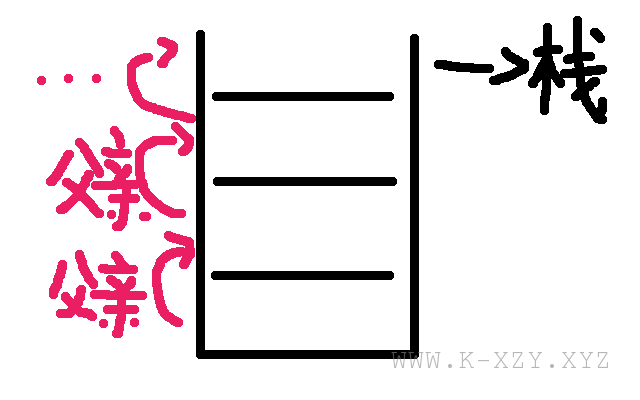
\includegraphics[width=0.5\textwidth]{images/vtree7.png} 
\caption{vtree7}
\end{figure}

首先我们在栈中添加节点 $1$。

然后接下来按照 DFS 序从小到达添加关键节点。

假如当前的节点与栈顶节点的 LCA 就是栈顶节点的话,则说明它们是在一条链上的。所以直接把当前节点入栈就行了。

\begin{figure}[h]
\centering
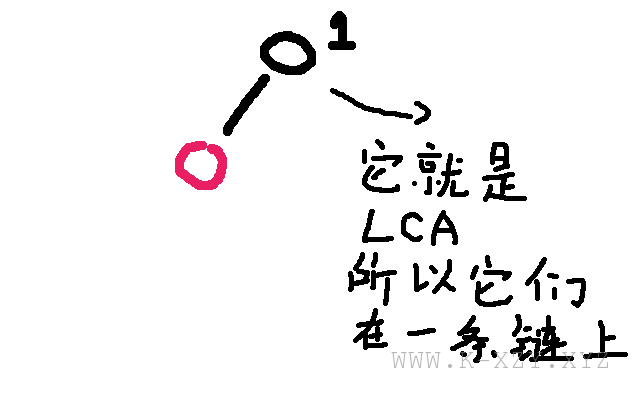
\includegraphics[width=0.5\textwidth]{images/vtree8.png} 
\caption{vtree8}
\end{figure}

假如当前节点与栈顶节点的 LCA 不是栈顶节点的话,比如这样——

\begin{figure}[h]
\centering
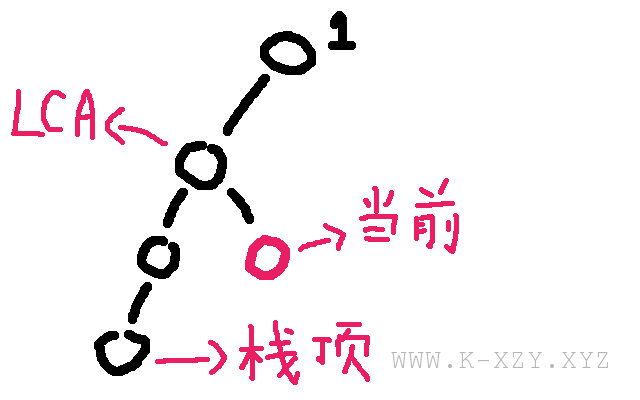
\includegraphics[width=0.5\textwidth]{images/vtree9.png} 
\caption{vtree9}
\end{figure}

那就…… 非常尴尬了

显然,当前单调栈维护的链是:

\begin{figure}[h]
\centering
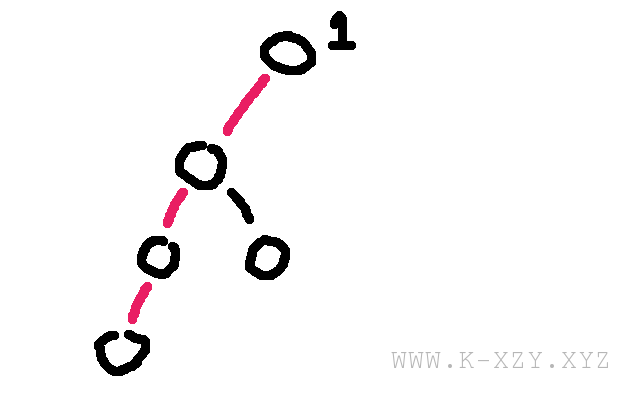
\includegraphics[width=0.5\textwidth]{images/vtree10.png} 
\caption{vtree10}
\end{figure}

而我们需要把链变成:

\begin{figure}[h]
\centering
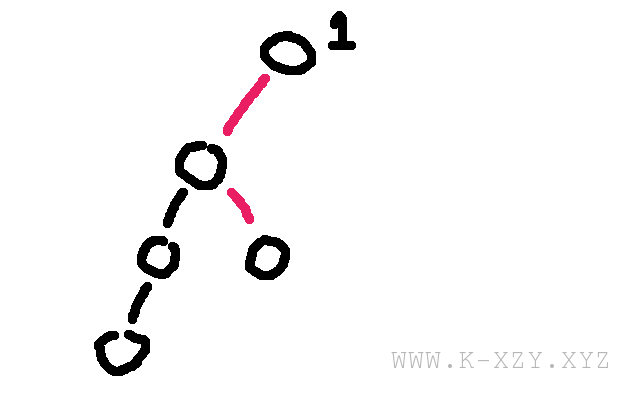
\includegraphics[width=0.5\textwidth]{images/vtree11.png} 
\caption{vtree11}
\end{figure}

那么我们就虚树中连上这些边:

\begin{figure}[h]
\centering
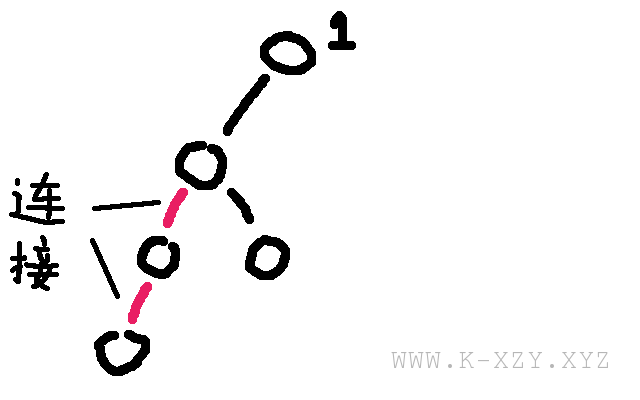
\includegraphics[width=0.5\textwidth]{images/vtree12.png} 
\caption{vtree11 (复件)}
\end{figure}

并且把这两个点从栈中弹出:

\begin{figure}[h]
\centering
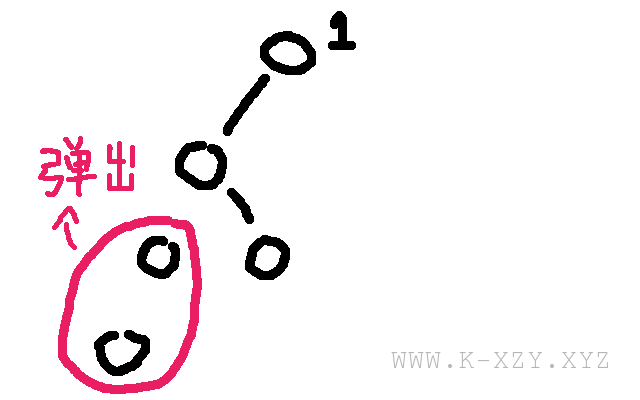
\includegraphics[width=0.5\textwidth]{images/vtree13.png} 
\caption{vtree13}
\end{figure}

假如弹出以后发现栈首不是 LCA 的话要让 LCA 入栈。

再把当前节点入栈就行了。

打个比方吧。

假如那棵树长这样:

\begin{figure}[h]
\centering
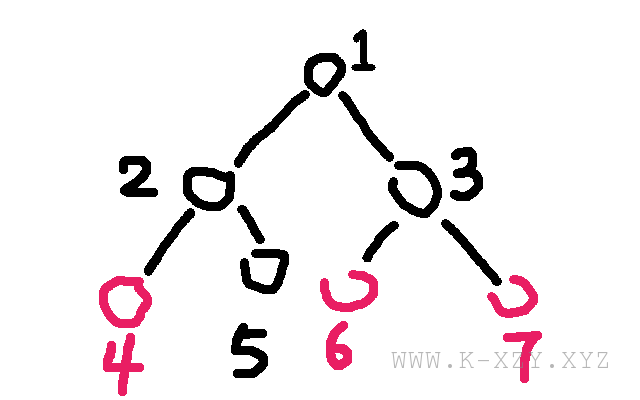
\includegraphics[width=0.5\textwidth]{images/vtree6.png} 
\caption{vtree6}
\end{figure}

那么步骤是这样的:

\begin{itemize}
\item 将 3 个关键点 $6,4,7$(我故意打乱了)按照 DFS 序排序,得到序列 $4,6,7$。
\item 将点 $1$ 入栈。
\item 取序列第一个作为当前节点,为 $4$。再取栈顶元素,为$1$。求$1$和$4$的$LCA$:$LCA(1,4)=1$。
\item 发现$LCA(1,4)=$栈顶元素,说明它们在虚树的一条链上,所以直接把当前节点$4$入栈,当前栈为$4,1$。
\item 取序列第二个作为当前节点,为 $6$。再取栈顶元素,为$4$。求$6$和$4$的$LCA$:$LCA(6,4)=1$。
\item 发现$LCA(6,4)\neq$栈顶元素,进入判断阶段。
\item 判断阶段:发现栈顶节点$4$的 DFS 序是大于$LCA(6,4)$的,但是次大节点(栈顶节点下面的那个节点)$1$的 DFS 序是等于$LCA$的(其实 DFS 序相等说明节点也相等),说明$LCA$已经入栈了,所以直接连接$1->4$的边,也就是$LCA$到栈顶元素的边。并把$4$从栈中弹出。
\item 结束了判断阶段,将$6$入栈,当前栈为$6,1$。
\item 取序列第三个作为当前节点,为$7$。再取栈顶元素,为$6$。求$7$和$6$的$LCA$:$LCA(7,6)=3$。
\item 发现$LCA(7,6)\neq$栈顶元素,进入判断阶段。
\item 判断阶段:发现栈顶节点$6$的 DFS 序是大于$LCA(7,6)$的,但是次大节点(栈顶节点下面的那个节点)$1$的 DFS 序是小于$LCA$的,说明$LCA$还没有入过栈,所以直接连接$3->6$的边,也就是$LCA$到栈顶元素的边。把$6$从栈中弹出,并且把$LCA(6,7)$入栈。
\item 结束了判断阶段,将$7$入栈,当前栈为$1,3,7$。
\item 发现序列里的 3 个节点已经全部加入过栈了,退出循环。
\item 此时栈中还有 3 个节点:$1, 3,7$,很明显它们是一条链上的,所以直接链接:$1->3$和$3->7$的边。
\item 虚树就建完啦!
\end{itemize}

其中有很多细节,比如我是用临接表存图的方式存虚树的,所以需要清空临接表。但是直接清空整个临接表是很慢的,所以我们在\textbf{有一个从未入栈的元素入栈的时候清空该元素对应的临接表}即可。

建立虚树的 C++ 代码大概长这样:

\begin{cppcode}
sort(h + 1, h + 1 + k, cmp);
sta[top = 1] = 1, g.sz = 0, g.head[1] = -1;
// 1号节点入栈,清空1号节点对应的临接表,设置临接表边数为1
for (int i = 1, l; i <= k; i += 1)
  if (h[i] != 1)  //如果1号节点是关键节点就不要重复添加
  {
    l = lca(h[i], sta[top]);  //计算当前节点与栈顶节点的LCA
    if (l !=
        sta[top])  //如果LCA和栈顶元素不同,则说明当前节点不再当前栈所存的链上
    {
      while (id[l] < id[sta[top - 1]])  //当次大节点的Dfs序大于LCA的Dfs序
        g.push(sta[top - 1], sta[top]),
            top--;  //把与当前节点所在的链不重合的链连接掉并且弹出
      if (id[l] >
          id[sta[top -
                 1]])  //如果LCA不等于次大节点(这里的大于其实和不等于没有区别)
        g.head[l] = -1, g.push(l, sta[top]), sta[top] = l;
      //说明LCA是第一次入栈,清空其临接表,连边后弹出栈顶元素,并将LCA入栈
      else
        g.push(l, sta[top--]);  //说明LCA就是次大节点,直接弹出栈顶元素
    }
    g.head[h[i]] = -1,
    sta[++top] = h[i];  //当前节点必然是第一次入栈,清空临接表并入栈
  }
for (int i = 1; i < top; i += 1)
  g.push(sta[i], sta[i + 1]);  //剩余的最后一条链连接一下
\end{cppcode}

于是我们就学会了虚树的建立了!

对于消耗战这题,直接在虚树上跑最开始讲的那个 DP 就行了,我们等于利用了虚树排除了那些没用的非关键节点!

\begin{itemize}
\item 若 $son[i]$ 不是关键点:$Dp[i]=Dp[i] + \min \{Dp[son[i]],w[i,son[i]]\}$
\item 若 $son[i]$ 是关键点:$Dp[i]=Dp[i] + w[i,son[i]]$
\end{itemize}

于是这题很简单就过了。

代码看下面。

\subsection{推荐习题}

\subsubsection{BZOJ - 2286 消耗战}

代码:

\begin{cppcode}
#include <bits/stdc++.h>

#define NS (250005)
#define LGS (18)

using namespace std;

typedef long long LL;

template <typename _Tp>
inline void IN(_Tp& dig) {
  char c;
  bool flag = 0;
  dig = 0;
  while (c = getchar(), !isdigit(c))
    if (c == '-') flag = 1;
  while (isdigit(c)) dig = dig * 10 + c - '0', c = getchar();
  if (flag) dig = -dig;
}

struct graph {
  int head[NS], nxt[NS << 1], to[NS << 1], w[NS << 1], sz;
  void init() { memset(head, -1, sizeof(head)), sz = 0; }
  graph() { init(); }
  void push(int a, int b, int c) {
    nxt[sz] = head[a], to[sz] = b, w[sz] = c, head[a] = sz++;
  }
  int& operator[](const int a) { return to[a]; }
} g;

int n, pre[NS][LGS + 1], dep[NS], mx[NS][LGS + 1], id[NS], dfn;

int m, k, h[NS], sta[NS], top, MX;

LL f[NS];

bool book[NS];

void Init(int a, int fa) {
  pre[a][0] = fa, dep[a] = dep[fa] + 1, id[a] = ++dfn;
  for (int i = 1; i <= LGS; i += 1) {
    pre[a][i] = pre[pre[a][i - 1]][i - 1];
    mx[a][i] = min(mx[a][i - 1], mx[pre[a][i - 1]][i - 1]);
  }
  for (int i = g.head[a]; ~i; i = g.nxt[i])
    if (g[i] != fa) mx[g[i]][0] = g.w[i], Init(g[i], a);
}

int lca(int a, int b) {
  MX = INT_MAX;
  if (dep[a] > dep[b]) swap(a, b);
  for (int i = LGS; i >= 0; i -= 1)
    if (dep[pre[b][i]] >= dep[a]) MX = min(MX, mx[b][i]), b = pre[b][i];
  if (a == b) return a;
  for (int i = LGS; i >= 0; i -= 1)
    if (pre[a][i] != pre[b][i]) {
      MX = min(MX, min(mx[a][i], mx[b][i]));
      a = pre[a][i], b = pre[b][i];
    }
  return pre[a][0];
}

bool cmp(int a, int b) { return id[a] < id[b]; }

void Dp(int a) {
  f[a] = 0;
  for (int i = g.head[a]; ~i; i = g.nxt[i]) {
    Dp(g[i]);
    if (book[g[i]])
      f[a] += g.w[i];
    else
      f[a] += min((LL)g.w[i], f[g[i]]);
  }
}

int main(int argc, char const* argv[]) {
  IN(n);
  for (int i = 1, a, b, c; i < n; i += 1)
    IN(a), IN(b), IN(c), g.push(a, b, c), g.push(b, a, c);
  Init(1, 0), IN(m);
  while (m--) {
    IN(k);
    for (int i = 1; i <= k; i += 1) IN(h[i]), book[h[i]] = 1;
    sort(h + 1, h + 1 + k, cmp);
    sta[top = 1] = 1, g.sz = 0, g.head[1] = -1;
    for (int i = 1, l; i <= k; i += 1)
      if (h[i] != 1) {
        l = lca(sta[top], h[i]);
        if (l != sta[top]) {
          while (id[l] < id[sta[top - 1]]) {
            lca(sta[top - 1], sta[top]);
            g.push(sta[top - 1], sta[top], MX);
            top--;
          }
          if (id[l] > id[sta[top - 1]]) {
            g.head[l] = -1, lca(l, sta[top]);
            g.push(l, sta[top], MX), sta[top] = l;
          } else
            lca(l, sta[top]), g.push(l, sta[top--], MX);
        }
        g.head[h[i]] = -1, sta[++top] = h[i];
      }
    for (int i = 1; i < top; i += 1)
      lca(sta[i], sta[i + 1]), g.push(sta[i], sta[i + 1], MX);
    Dp(1), printf("%lld\n", f[1]);
    for (int i = 1; i <= k; i += 1) book[h[i]] = 0;
  }
  return 0;
}
\end{cppcode}

\subsubsection{BZOJ - 3611 大工程}

代码:

\begin{cppcode}
#include <bits/stdc++.h>

#define NS (1000005)
#define LGS (20)

#define INF (100000000)

using namespace std;

typedef long long LL;

template <typename _Tp>
inline void IN(_Tp& dig) {
  char c;
  bool flag = 0;
  dig = 0;
  while (c = getchar(), !isdigit(c))
    if (c == '-') flag = 1;
  while (isdigit(c)) dig = dig * 10 + c - '0', c = getchar();
  if (flag) dig = -dig;
}

struct graph {
  int head[NS], nxt[NS << 1], to[NS << 1], sz;
  void init() { memset(head, -1, sizeof(head)), sz = 0; }
  graph() { init(); }
  void push(int a, int b) { nxt[sz] = head[a], to[sz] = b, head[a] = sz++; }
  int operator[](const int a) { return to[a]; }
} g;

int n, id[NS], dfn, q, k, h[NS], sz[NS], mn[NS], mx[NS], mnans, mxans;

int pre[NS][LGS + 1], dep[NS];

int sta[NS], top;

bool book[NS];

LL f[NS], tot;

void Init(int a, int fa) {
  pre[a][0] = fa, dep[a] = dep[fa] + 1, id[a] = ++dfn;
  for (int i = 1; i <= LGS; i += 1) pre[a][i] = pre[pre[a][i - 1]][i - 1];
  for (int i = g.head[a]; ~i; i = g.nxt[i])
    if (g[i] != fa) Init(g[i], a);
}

int lca(int a, int b) {
  if (dep[a] > dep[b]) swap(a, b);
  for (int i = LGS; i >= 0; i -= 1)
    if (dep[pre[b][i]] >= dep[a]) b = pre[b][i];
  if (a == b) return a;
  for (int i = LGS; i >= 0; i -= 1)
    if (pre[a][i] != pre[b][i]) a = pre[a][i], b = pre[b][i];
  return pre[a][0];
}

bool cmp(int a, int b) { return id[a] < id[b]; }

void Dp(int a) {
  sz[a] = book[a], f[a] = 0;
  if (book[a])
    mn[a] = mx[a] = 0;
  else
    mn[a] = INF, mx[a] = -INF;
  for (int i = g.head[a], l; ~i; i = g.nxt[i]) {
    Dp(g[i]), l = dep[g[i]] - dep[a];
    tot += (f[a] + sz[a] * l) * sz[g[i]] + f[g[i]] * sz[a];
    sz[a] += sz[g[i]], f[a] += f[g[i]] + l * sz[g[i]];
    mnans = min(mnans, mn[a] + mn[g[i]] + l);
    mxans = max(mxans, mx[a] + mx[g[i]] + l);
    mn[a] = min(mn[a], mn[g[i]] + l);
    mx[a] = max(mx[a], mx[g[i]] + l);
  }
}

int main(int argc, char const* argv[]) {
  IN(n);
  for (int i = 1, a, b; i < n; i += 1) IN(a), IN(b), g.push(a, b), g.push(b, a);
  Init(1, 0), IN(q);
  while (q--) {
    IN(k);
    for (int i = 1; i <= k; i += 1) IN(h[i]), book[h[i]] = 1;
    sort(h + 1, h + 1 + k, cmp);
    sta[top = 1] = 1, g.sz = 0, g.head[1] = -1;
    for (int i = 1, l; i <= k; i += 1)
      if (h[i] != 1) {
        l = lca(h[i], sta[top]);
        if (l != sta[top]) {
          while (id[l] < id[sta[top - 1]])
            g.push(sta[top - 1], sta[top]), top--;
          if (id[l] > id[sta[top - 1]])
            g.head[l] = -1, g.push(l, sta[top]), sta[top] = l;
          else
            g.push(l, sta[top--]);
        }
        g.head[h[i]] = -1, sta[++top] = h[i];
      }
    for (int i = 1; i < top; i += 1) g.push(sta[i], sta[i + 1]);
    mnans = INF, mxans = -INF, tot = 0, Dp(1);
    printf("%lld %d %d\n", tot, mnans, mxans);
    for (int i = 1; i <= k; i += 1) book[h[i]] = 0;
  }
  return 0;
}
\end{cppcode}

\subsubsection{CF613D Kingdom and its Cities}

代码:

\begin{cppcode}
#include <bits/stdc++.h>

#define NS (100005)
#define LGS (17)

using namespace std;

template <typename _Tp>
inline void IN(_Tp& dig) {
  char c;
  bool flag = 0;
  dig = 0;
  while (c = getchar(), !isdigit(c))
    if (c == '-') flag = 1;
  while (isdigit(c)) dig = dig * 10 + c - '0', c = getchar();
  if (flag) dig = -dig;
}

struct graph {
  int head[NS], nxt[NS << 1], to[NS << 1], sz;
  void init() { memset(head, -1, sizeof(head)), sz = 0; }
  graph() { init(); }
  void push(int a, int b) { nxt[sz] = head[a], to[sz] = b, head[a] = sz++; }
  int operator[](const int a) { return to[a]; }
} g;

int n, id[NS], dfn, q, k, h[NS], c[NS];

int pre[NS][LGS + 1], dep[NS];

int sta[NS], top;

bool book[NS];

void Init(int a, int fa) {
  pre[a][0] = fa, dep[a] = dep[fa] + 1, id[a] = ++dfn;
  for (int i = 1; i <= LGS; i += 1) pre[a][i] = pre[pre[a][i - 1]][i - 1];
  for (int i = g.head[a]; ~i; i = g.nxt[i])
    if (g[i] != fa) Init(g[i], a);
}

int lca(int a, int b) {
  if (dep[a] > dep[b]) swap(a, b);
  for (int i = LGS; i >= 0; i -= 1)
    if (dep[pre[b][i]] >= dep[a]) b = pre[b][i];
  if (a == b) return a;
  for (int i = LGS; i >= 0; i -= 1)
    if (pre[a][i] != pre[b][i]) a = pre[a][i], b = pre[b][i];
  return pre[a][0];
}

bool cmp(int a, int b) { return id[a] < id[b]; }

int Dp(int a) {
  int tot = 0, ans = 0;
  for (int i = g.head[a]; ~i; i = g.nxt[i]) ans += Dp(g[i]), tot += c[g[i]];
  if (book[a])
    c[a] = 1, ans += tot;
  else if (tot > 1)
    c[a] = 0, ans++;
  else
    c[a] = tot;
  return ans;
}

int main(int argc, char const* argv[]) {
  IN(n);
  for (int i = 1, a, b; i < n; i += 1) IN(a), IN(b), g.push(a, b), g.push(b, a);
  Init(1, 0), IN(q);
  while (q--) {
    IN(k);
    for (int i = 1; i <= k; i += 1) IN(h[i]), book[h[i]] = 1;
    for (int i = 1; i <= k; i += 1)
      if (book[pre[h[i]][0]]) {
        puts("-1");
        goto end;
      }
    sort(h + 1, h + 1 + k, cmp);
    sta[top = 1] = 1, g.sz = 0, g.head[1] = -1;
    for (int i = 1, l; i <= k; i += 1)
      if (h[i] != 1) {
        l = lca(h[i], sta[top]);
        if (l != sta[top]) {
          while (id[l] < id[sta[top - 1]])
            g.push(sta[top - 1], sta[top]), top--;
          if (id[l] > id[sta[top - 1]])
            g.head[l] = -1, g.push(l, sta[top]), sta[top] = l;
          else
            g.push(l, sta[top--]);
        }
        g.head[h[i]] = -1, sta[++top] = h[i];
      }
    for (int i = 1; i < top; i += 1) g.push(sta[i], sta[i + 1]);
    printf("%d\n", Dp(1));
  end:
    for (int i = 1; i <= k; i += 1) book[h[i]] = 0;
  }
  return 0;
}
\end{cppcode}

\subsubsection{BZOJ - 3572 世界树}

(丧心病狂啊)

代码:

\begin{cppcode}
#include <bits/stdc++.h>

#define NS (300005)
#define LGS (19)
#define FIR first
#define SEC second

using namespace std;

typedef pair<int, int> PII;

template <typename _Tp>
inline void IN(_Tp& dig) {
  char c;
  bool flag = 0;
  dig = 0;
  while (c = getchar(), !isdigit(c))
    if (c == '-') flag = 1;
  while (isdigit(c)) dig = dig * 10 + c - '0', c = getchar();
  if (flag) dig = -dig;
}

struct graph {
  int head[NS], nxt[NS << 1], to[NS << 1], sz;
  void init() { memset(head, -1, sizeof(head)), sz = 0; }
  graph() { init(); }
  void push(int a, int b) { nxt[sz] = head[a], to[sz] = b, head[a] = sz++; }
  int operator[](const int a) { return to[a]; }
} g;

int n, m, q, h[NS], arr[NS], ans[NS];

int pre[NS][LGS + 1], dep[NS], id[NS], dfn, sz[NS];

int st[NS], top;

bool book[NS];

PII mx[NS];

bool cmp(int a, int b) { return id[a] < id[b]; }

void Init(int a, int fa) {
  pre[a][0] = fa, dep[a] = dep[fa] + 1, id[a] = ++dfn, sz[a] = 1;
  for (int i = 1; i <= LGS; i += 1) pre[a][i] = pre[pre[a][i - 1]][i - 1];
  for (int i = g.head[a]; ~i; i = g.nxt[i])
    if (g[i] != fa) Init(g[i], a), sz[a] += sz[g[i]];
}

int jump(int a, int k) {
  for (int i = 0; i <= LGS; i += 1)
    if ((k >> i) & 1) a = pre[a][i];
  return a;
}

int lca(int a, int b) {
  if (dep[a] > dep[b]) swap(a, b);
  b = jump(b, dep[b] - dep[a]);
  if (a == b) return a;
  for (int i = LGS; i >= 0; i -= 1)
    if (pre[a][i] != pre[b][i]) a = pre[a][i], b = pre[b][i];
  return pre[a][0];
}

void dfs1(int a) {
  if (book[a])
    mx[a] = PII(0, a);
  else
    mx[a] = PII(1e8, 0);
  for (int i = g.head[a]; ~i; i = g.nxt[i]) {
    dfs1(g[i]);
    PII tmp = mx[g[i]];
    tmp.FIR = dep[mx[g[i]].SEC] - dep[a];
    mx[a] = min(mx[a], tmp);
  }
}

void dfs2(int a) {
  for (int i = g.head[a]; ~i; i = g.nxt[i]) {
    PII tmp = mx[a];
    tmp.FIR += dep[g[i]] - dep[a];
    mx[g[i]] = min(mx[g[i]], tmp), dfs2(g[i]);
  }
  ans[mx[a].SEC] = max(ans[mx[a].SEC], sz[a]);
}

void dfs3(int a) {
  for (int i = g.head[a], x, y, dis, z; ~i; i = g.nxt[i]) {
    if (x = mx[a].SEC, y = mx[g[i]].SEC, x != y) {
      dis = dep[x] + dep[y] - (dep[lca(x, y)] << 1);
      z = jump(g[i], (dis >> 1) - mx[g[i]].FIR);
      if (dis & 1)
        ans[x] -= sz[z];
      else {
        if (z != a && z != g[i])
          z = jump(g[i], (dis >> 1) - mx[g[i]].FIR - (x < y));
        else if (z == a)
          z = jump(g[i], (dis >> 1) - mx[g[i]].FIR - 1);
        ans[x] -= sz[z];
      }
      if (g[i] != z) ans[y] += sz[z] - sz[g[i]];
    }
    dfs3(g[i]);
  }
}

int main(int argc, char const* argv[]) {
  IN(n);
  for (int i = 1, a, b; i < n; i += 1) IN(a), IN(b), g.push(a, b), g.push(b, a);
  Init(1, 0), IN(q);
  while (q--) {
    IN(m), g.sz = 0;
    for (int i = 1; i <= m; i += 1)
      IN(h[i]), book[h[i]] = 1, ans[arr[i] = h[i]] = 0;
    sort(h + 1, h + 1 + m, cmp), st[top = 1] = 1, g.head[1] = -1;
    for (int i = 1, l; i <= m; i += 1) {
      if (h[i] == 1) continue;
      l = lca(st[top], h[i]);
      if (l != st[top]) {
        while (id[l] < id[st[top - 1]]) g.push(st[top - 1], st[top]), top--;
        if (id[l] > id[st[top - 1]])
          g.head[l] = -1, g.push(l, st[top]), st[top] = l;
        else
          g.push(l, st[top--]);
      }
      g.head[h[i]] = -1, st[++top] = h[i];
    }
    for (int i = 1; i < top; i += 1) g.push(st[i], st[i + 1]);
    dfs1(1), dfs2(1), dfs3(1);
    for (int i = 1; i <= m; i += 1) printf("%d ", ans[arr[i]]);
    putchar(10);
    for (int i = 1; i <= m; i += 1) book[h[i]] = 0;
  }
  return 0;
}
\end{cppcode}
